\section*{Assignment 1}
% Installing VA testbacnhes.

\begin{itemize}
    \item Installing \& get acquainted with the lab environment (virtual machine)
    \item differences between combinatorial and sequential logic and how to implement in Verilog guided by some examples (halfadder, counter)
    \item simulation and testing in ISE
\end{itemize}

%\emph{Aufgabe: }Nach eingien einführenden Aufgabe, sollten wir einen UART Transmitter, dann einen UART-Reciver, und abschließend um beide miteinander zu Kombinieren Ein Echo auf dem FPGI zu Implementieren.

After some small introducing assignments we were asked to implement an UART-transmitter and an UART-reciver and test them via test bench. Afterwards we should combine these two to implement an echo on the FPGI.


%\emph{Bearbeitung und Lösung: }Der Empfänger hat 3 Zustände $z_0$, $z_1$, $z_2$.
The UART-reciver has three different states $z_0$, $z_1$, $z_2$.
\begin{itemize}


\item[$z_0$:] Initial state: Waiting for falling/rising edge, which is showing the begin of an UART communication.
%Ausgangszustand warten auf fallende/steigende Flanke, die den Beginn der seriellen UART Kommunikation anzeigt.
\item[$z_1$:] Receiving state: For every bit you have to wait the appropriate time according to the transfer rate, until you can read the next bit. The individual bits read will be saved to a byte array. After saving a bit yo have to shift all the bit in the array, so the next read Bit can be saved to the 1st position.
%Empfangszustand: Für jedes Bit muss entsprechend der Übertragungsrate gewartet werden, bis das nächste gelesen werden kann. Die eingelesenen einzel Bits werden in einem Byte Array gespeichert, dass nach speichern eines Wertes ein Bit geshiftet wird, um das nächste Bit zu speichern. 
\item[$z_2$:] Stop state: In this state the bit-string will be reset to its initial state. Furthermore, the valid bit will be set, to show that the saved byte can be read through the output.
%im Stoppzustand wird der Bit-String wieder in den Augangszustand versetzt, außerdem wird Valid-Bit gestezt. Das heißt, dass das Byte nun ausgelesen werden kann (am Output anliegt). 
\end{itemize}

%\emph{Bearbeitung und Lösung: }Der Sender hat 4 Zustände $z_0$, $z_1$, $z_2$, $z_3$.
The UART-transmitter got four states $z_0$, $z_1$, $z_2$, $z_3$.
\begin{itemize}


\item[$z_0$:] Initial state: In the initial state, the transmitter is waiting for an enable. The Output is set to \verb+0+.
%Ausgangszustand wartet auf enable. Ausgabe ist auf 0.
\item[$z_1$:] Sending state: The output will be set to the value of the zeroth bit of an 8-bit string. Furthermore, all the bits of the 8-bit string will be shifted by one position.
%Die Augabe, wird dem 0. Bit eines 8-Bit Strings gleichgesetzt und das 8-Bit Sting wird um eine Stelle verschoben.
\item[$z_2$:] Checking state: in this state will be checked if the byte where shifted 8 times. If not, the transmitter will go back in sending state. If yes, the transmitter will go into the finished state.
%Nachdem 8 Bits ausgelesen, bzw. gesendet wurden Wird der vorgang beendet.
\item[$z_3$:] Finished state: in this state the byte was fully transmitted and rdy will be set to 1 to show, that the transmitter is ready to send new data.
%rdy wird auf 1 gesetzt, um anzuzeigen, das er bereit ist neue Daten zu senden.  

\end{itemize}\newpage

\begin{figure}[h!]
    \begin{center}
%        \hrule\vspace{1em}
        \usetikzlibrary{arrows.meta}
\usetikzlibrary{calc,intersections,through,backgrounds}
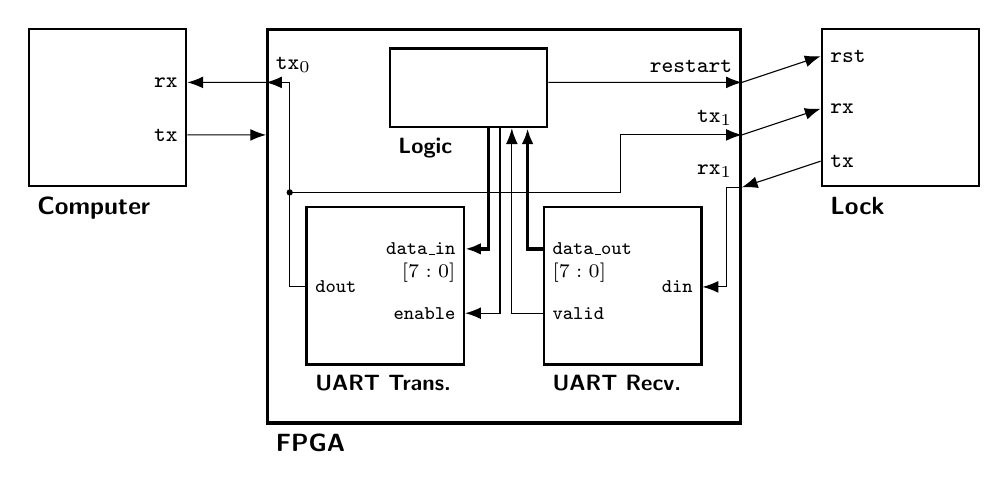
\begin{tikzpicture}
% 	\tikzset{
% 	  every node/.style={scale=1.1}
% 	}	
	\tikzset{comp/.style={
		rectangle, draw=black, thick
	}}	
	\tikzset{component/.style={
		comp, minimum width=6cm, minimum height=5cm, very thick
	}}
	\tikzset{component_small/.style={
		comp, minimum width=2cm, minimum height=2cm, thick
	}}
	\tikzset{caption/.style={
		below right
	}}
	\tikzset{conn/.style={
		-{Latex[length=2mm]}
	}}
	
	% FPGA
	\node (FPGA) [component] at (0,0) {}
		% Caption
		node [caption] at (FPGA.south west) { \small{\textsf{\textbf{FPGA}}} }
		
		% In/-outputs links
		coordinate [yshift=3cm+0.4pt+0.666cm, label={ above right : \footnotesize{} }]                           (FPGA_rx0) at (FPGA.south west) % unten
		coordinate [yshift=3cm+0.4pt+1.333cm, label={ above right : \footnotesize{$\texttt{tx}_0$} }] (FPGA_tx0) at (FPGA.south west) % oben

		% In/outputs  rechts
		coordinate [yshift=3cm+0.4pt,                    label={ above left : \footnotesize{$\texttt{rx}_1$} }]      (FPGA_rx1)       at (FPGA.south east)  % unten
		coordinate [yshift=3cm+0.4pt+0.666cm, label={ above left : \footnotesize{$\texttt{tx}_1$} }]      (FPGA_tx1)       at (FPGA.south east) % mitte
		coordinate [yshift=3cm+0.4pt+1.333cm, label={ above left : \footnotesize{$\texttt{restart}$} }] (FPGA_restart) at (FPGA.south east) % oben
	;

	% Logic
	\node (Logic) at (FPGA.north) [comp, minimum height=1cm, minimum width=2cm, below, shift={(-0.45cm, -0.25cm)}] {}
		node [caption] at (Logic.south west) { \textsf{\footnotesize{\textbf{Logic}}} }
	;

	% Receiver
	\node (Receiver) at (FPGA.south east) [component_small, above left, shift={(-0.5, 0.75)}] {}
		% Caption
		node [caption] at (Receiver.south west) { \textsf{\footnotesize{\textbf{UART Recv.}}} }

		% Input rechts
		coordinate [yshift=1cm, label={ left : \scriptsize{\texttt{din}} }] (Receiver_din) at (Receiver.south east)

		% Outpus links
		coordinate [yshift=0.666cm,                 label={ right : \scriptsize{\texttt{valid}} }]           (Receiver_valid)           at (Receiver.south west) % unten
		coordinate [yshift=1.333cm+0.15cm, label={ right : \scriptsize{\texttt{data\_out}} }] (Receiver_data_out)    at (Receiver.south west) % oben
		coordinate [yshift=1.333cm-0.15cm,  label={ right : \scriptsize{$[7:0]$} }]                     (Receiver_data_out2) at (Receiver.south west) % mitte
	;

	% Transmitter
	\node (Transmitter) at (FPGA.south west) [component_small, above right, shift={(0.5, 0.75)}] {}
		node [caption] at (Transmitter.south west) { \textsf{\footnotesize{\textbf{UART Trans.}}} }

		% Output links
		coordinate [yshift=1cm, label={ right: \scriptsize{\textsf{\texttt{dout}}} }] (Transmitter_dout) at (Transmitter.south west) % unten

		% Inputs links
		coordinate [yshift=0.666cm,                 label={ left : \scriptsize{\texttt{enable}} }]    (Transmitter_enable)   at (Transmitter.south east) % unten
		coordinate [yshift=1.333cm-0.15cm,  label={ left : \scriptsize{$[7:0]$} }]                  (Transmitter_data_in2)at (Transmitter.south east) % mitte
		coordinate [yshift=1.333cm+0.15cm, label={ left : \scriptsize{\texttt{data\_in}} }] (Transmitter_data_in)  at (Transmitter.south east) % oben	
	;

	% Computer
	\node (Computer) [component_small, below left, xshift=-1cm] at (FPGA.north west) {}
		% Caption
		node [caption] at (Computer.south west) { \small{\textsf{\textbf{Computer}}} }

		% In/outputs rechts
		coordinate [yshift=0.666cm, label={ left:\footnotesize{\texttt{tx}} }] (Computer_tx) at (Computer.south east) % unten
		coordinate [yshift=1.333cm, label={ left:\footnotesize{\texttt{rx}} }] (Computer_rx) at (Computer.south east) % oben
	;

	% Lock
	\node (Lock) [component_small, below right, xshift=1cm] at (FPGA.north east) {}
		% Caption
		node [caption] at (Lock.south west) { \small{\textsf{\textbf{Lock}}} }

		% In/outputs rechts
		coordinate [yshift=0.333cm, label={ right:\footnotesize{\texttt{tx}} }]   (Lock_tx)   at (Lock.south west) % unten
		coordinate [yshift=0.999cm, label={ right:\footnotesize{\texttt{rx}} }]   (Lock_rx)   at (Lock.south west) % mitte
		coordinate [yshift=1.666cm, label={ right:\footnotesize{\texttt{rst}} }] (Lock_rst)  at (Lock.south west) % oben
	;

	% Computer <-> FPGA
	\draw[conn]  (FPGA_tx0) -- (Computer_rx);
	\draw[conn] (Computer_tx) -- (FPGA_rx0);

	% FPGA <-> Lock
	\draw[conn] (FPGA_restart) -- (Lock_rst);
	\draw[conn] (FPGA_tx1) -- (Lock_rx);
	\draw[conn] (Lock_tx) -- (FPGA_rx1) ;
	
	% FPGA internal
		\draw[conn] ([yshift=0.583cm] Logic.south east) -- (FPGA_restart);
	
		% Connections to/from Receiver
		\draw[conn] (FPGA_rx1) -- ([xshift=-0.2cm] FPGA_rx1) |- (Receiver_din);
		\draw[conn, very thick] (Receiver_data_out) -| ([xshift=0.75cm] Logic.south); 
		\draw[conn] (Receiver_valid) -| ([xshift=0.55cm] Logic.south);
		
		% Connections to/from Transmitter
		\draw[conn, very thick] ([xshift=0.25cm]Logic.south) |- (Transmitter_data_in);
		\draw[conn] ([xshift=0.4cm] Logic.south) |- (Transmitter_enable);
		\draw[conn, name path=Transmitter_dout--FPGA_tx0] (Transmitter_dout) -- ([xshift=-0.2cm] Transmitter_dout) |- (FPGA_tx0);
		\draw[conn, name path=Transmitter_dout--FPGA_tx1] ([shift={(-0.2cm, 1.2cm)}] Transmitter_dout) -- ([shift={(4cm, 1.2cm)}] Transmitter_dout) |- (FPGA_tx1);

		% Intersection
		\fill[name intersections={of=Transmitter_dout--FPGA_tx0 and Transmitter_dout--FPGA_tx1, total=\t}] (intersection-\t) circle (0.4mm);
\end{tikzpicture}
        \caption{Timing attack.}
        \label{fig:as5-schematic}
        \vspace{1em}\hrule
    \end{center}
\end{figure}
